\begin{frame}{Free Fermion Edge Classification}
\vskip-1.5cm
\only<1>{
By partitioning the wavefunction, we can glimpse the edge
\begin{columns}[T]
\begin{column}{0.5\textwidth}
\begin{figure}
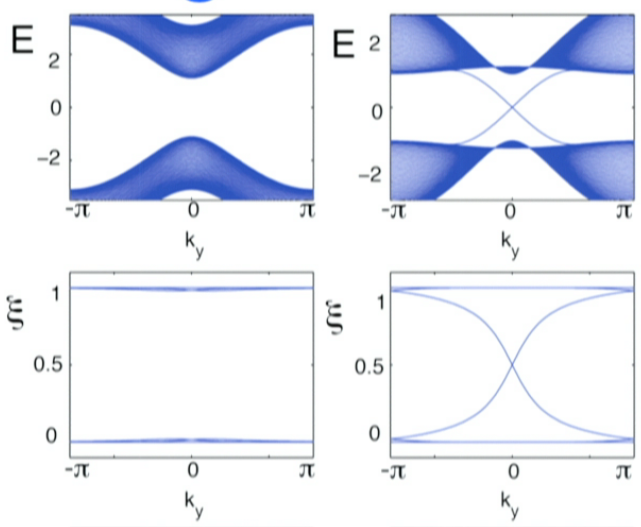
\includegraphics[width=\linewidth]{diagrams/QSH.png}
\caption{Top: Physical spectrum with boundary.
Bottom: 'Single particle entanglement spectrum'}
\end{figure}
\end{column}
\begin{column}{0.5\textwidth}
\bi
\item $G_{ij} = \ev{c^{\dagger}_i c_j}$ 
%\item Determines free fermion state
%\item Eigenvalues are 1, 0
\item $G^L_{ij}$ is G restricted to left half of cylinder
\item Spectrum of $G^L$ shown.
\item 'Gapless entanglement mode' protected by $\mathcal{T}$

\item Bulk wavefunction E.S. shown to capture edge physics
\item Bulk wavefunction shown to be distinct from atomic insulator
\ei 

\end{column}
\end{columns}
}
\only<2>{
    Results for free fermions without lattice symmetries:
    \begin{figure}
    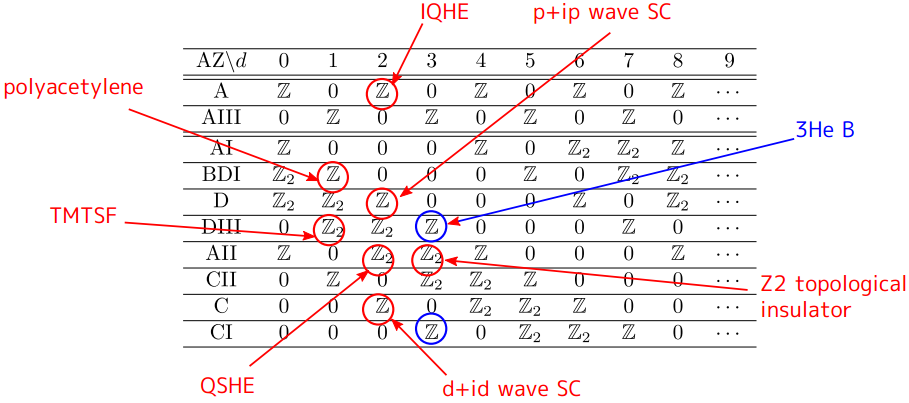
\includegraphics[width=\linewidth]{diagrams/AZ.png}
    \caption{Free-fermion classification (ten-fold way) for $       \mathcal{T}, \mathcal{C}$} 
    \end{figure}
    \footnotetext[5]{
    \citep{Ryu2009-qc}} 
%These invariants aren't always very physical, and while they distinguish free fermion Hamiltonians, they aren't guaranteed to stick around when you add interactions.

% Most of the invariants are only well defined in the presence of some additional symmetry

% There is an big table of free-fermion classification called the 10 fold way for time-reversal and charge conjugation symmetry, and a bigger table when you include lattice symmetries (Topological Crystalline Insulators)
}


\end{frame}